\documentclass[10pt,legal]{article} % Paper type (a4paper, usletter or legal) and font size (10, 11 or 12)

\setlength\topmargin{-48pt} % Top margin
\setlength\headheight{0pt} % Header height
\setlength\textwidth{7.0in} % Text width
\setlength\textheight{9.5in} % Text height
\setlength\oddsidemargin{-30pt} % Left margin
\setlength\evensidemargin{-30pt} % Left margin (even pages) - only relevant with 'twoside' article option

\usepackage{charter} % Charter font for main content

\frenchspacing % Reduces space after periods to make text more compact for a three-column layout

\usepackage{graphicx} % Required for including images
\usepackage{amssymb,amsmath} % Math packages
\usepackage{multicol} % Required for the three-column layout of the document
\usepackage{url} % Clickable links
\usepackage{enumitem} % Reduces the amount of space within and between lists with [noitemsep,nolistsep]
\usepackage{marvosym} % Required for the use of symbols
\usepackage{wrapfig} % Allows wrapping text around figures
\usepackage[T1]{fontenc} % Use 8-bit encoding that has 256 glyphs
\usepackage{datetime} % Required for defining a custom date style
\newdateformat{mydate}{\monthname[\THEMONTH] \THEYEAR} % Set a custom date format
\usepackage[pdfpagemode=FullScreen, colorlinks=false]{hyperref} % Link colors and PDF behavior in Acrobat
\usepackage{fancyhdr} % Required to define custom headers/footers
\pagestyle{fancy} % Enables the custom headers/footers for all pages following this
\cfoot{} % Empty center footer
\renewcommand{\headrulewidth}{0.0pt} % No horizontal rule for the header
\renewcommand{\footrulewidth}{0.1pt} % Horizontal rule separating the footer from the document
\newcommand{\HorRule}[1]{\noindent\rule{\linewidth}{#1}} % Creates a horizontal rule
\newcommand{\SepRule}{\noindent	% Creates a shorter separator rule
}
\newcommand{\NewsletterName}[1]{ % Newsletter title
\begin{center}
\huge \usefont{T1}{fvs}{b}{n} % Use the Bera Sans Bold font
#1
\end{center}	
\par \normalsize \normalfont}

\newcommand{\JournalIssue}[1]{ % Date and issue number at the top of the newsletter
\hfill \textsc{\mydate \today, No #1} % Right-aligned date and issue number
\par \normalsize \normalfont}

\newcommand{\NewsItem}[1]{ % News item title
\usefont{T1}{fvs}{n}{n} % Use the Bera Sans Normal font
\vspace{24pt}\large #1\vspace{3pt} % Print the title with space around it in a larger font size
\par \normalsize \normalfont}

\newcommand{\NewsAuthor}[1]{ % Author name under the item title
\hfill by \textsc{#1} \vspace{10pt} % Right-aligned author name in small caps with space after it
\par \normalfont}

\begin{document}

\NewsletterName{Complexity Results in Epistemic Planning} % Newsletter title

\noindent\HorRule{2pt} \\[-0.75\baselineskip] % Thick horizontal rule
\HorRule{0.5pt} % Thin horizontal rule

\begin{multicols}{2} % Begin the three-column layout

\NewsItem{Paper Summary  \cite{2014arXiv1404.0844A} }
\NewsAuthor{Prabath Peiris}

The primary focus of AI is the development of rational, autonomous agents. In the field of automated planning, these agents should exhibit goal-directed behavior. In Automated planning, there is a planning task that consists of initial state, the finite set of actions and the goal formula. The aim is to compute a plan that is a sequence of actions which leads to goal formula starting from the initial state. In this planning, the domain models employed are formulated using propositional logic. However, when we reach more complex settings such as multi-agent domains, such models come up short due to the limited expressive power of propositional logic. To overcome this limitation, the Epistemic Planning is being used. Epistemic Planning is where agents can reason about their own and other agents' beliefs as part of the planning process. For example, in games with strong epistemic components would be what will the other agents know if I choose to announce that I have this card? or in robotics "Fetch a cup of tea, the leafs are in the cupboard". 
This paper \cite{2014arXiv1404.0844A}  establishes a framework for epistemic planning based on Dynamic Epistemic Logic (DEL). From classical planning to epistemic planning, the propositional logic replaces by DEL. 
\begin{center}
\small
\begin{tabular}{ |p{1cm}|p{3.1cm}|p{3.2cm} |} 
 \hline
  & Classical planning & Epistemic planning \\ \hline
 States & models of prop. logic &  models of MA epist. logic \\\hline
Goal formula & formula of prop. logic & formula of MA epist. logic \\ \hline
Actions & induced by action schemas &  action models of DEL \\
 \hline
\end{tabular}
\end{center}
Epistemic planning task is the planning task in epistemic planning and Planing existence for a class of epistemic planning tasks X: "Given a planning task in X, does there exist a plan for it?". In this paper complexity results for the plan existence problem for various classes of epistemic planning tasks.

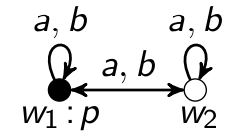
\includegraphics[width=0.1\textwidth]{initialstate.png}
\par\small\textit{Figure 1: Initial State}
\\
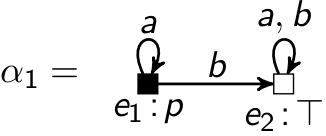
\includegraphics[width=0.15\textwidth]{a1.png}
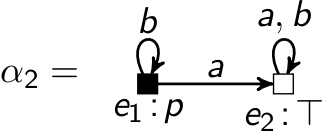
\includegraphics[width=0.15\textwidth]{a2.png}
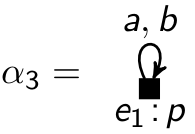
\includegraphics[width=0.1\textwidth]{a3.png} 
\par\small\textit{Figure 2: Actions}\\
For example, we can consider the epistemic planning tasks with initial state (Figure 1) and actions (Figure 2). $\alpha_1$ privately announcing $p$ to $a$,  $\alpha_2$: privately announcing $p$ to $b$; $\alpha_3$: publicly announcing $p$ to both agents. The Goal formula is defined as:
\begin{equation}
K_a P \wedge	 K_b p \wedge	 \neg K_a K_b p \wedge  \neg K_b K_a p
\end{equation}

A plan for this task is $\alpha_1$, $\alpha_2$. Another plan is $\alpha_2$, $\alpha_1$. Also, $\alpha_1$, $\alpha_2$, $\alpha_1$ and $\alpha_1$, $\alpha_1$, $\alpha_2$ are plans, etc. Actions are graphs. Different graph structures allow different actions to be formed. We study how the underlying graph structure impact complexity of plan existence. Summary of complexity results for plan existence. Summary of complexity results for plan existence (Table 1) \cite{e4e604b96afd4002b1aef671f4ffa495}
\begin{center}
\vspace{1pt}
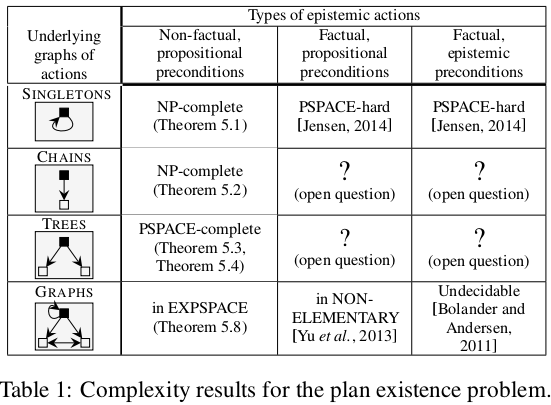
\includegraphics[width=1.0\linewidth]{complexity.png} % Example of an image taking up the total width of the page
\vspace{1pt}
\end{center}
There are reasons to study the complexity of very restrictive of epistemic planning are this is relevant to many interesting applications, and to understand where does the complexity come from and constructing search heuristics for planning engines (relaxed problems)

Since propositional STRIPS planning is PSPACE-complete, efficient planning systems have used relaxed
planning tasks to compute precise heuristics efficiently. For instance, the highly influential Fast-Forward planning system relaxes planning tasks by ignoring delete lists. This paper contribution here show restrictions on the graphs underlying epistemic actions crucially affect computational complexity. This, in the combination with restrictions on preconditions and postconditions (factual change), provides a platform for investigating (tractable) relaxations of epistemic planning tasks, and hence for the development of efficient epistemic planning systems.
\bibliography{articles}{}
\bibliographystyle{plain}
\end{multicols}
\end{document} 